\section{\MakeUppercase{Implementation Details}}
The project is developed using Python, leveraging PyTorch as the primary deep learning framework. Interactive Python sessions are utilized for testing and rapid prototyping. Jupyter Notebooks are employed for exploratory data analysis and iterative experimentation, allowing for an interactive and visual approach to model development. TensorBoard is used to visualize training metrics and monitor the performance of the \gls{siren} network during training. Visual Studio Code serves as the main \gls{ide} for code writing and debugging.

\subsection{Instrumentation}
    The software and hardware used for this project are listed below:
    \begin{table}[H]
        \caption{Instrumentation Table}
        \label{table:instrumentation-table}
        \centering
        \begin{tabular}{|L{0.2\linewidth}|L{0.3\linewidth}|L{0.4\linewidth}|}
            \hline
            \textbf{Requirement} & \textbf{Solution} & \textbf{Reason} \\
            \hline
            High-Performance Computing & NVIDIA RTX 4090 & Overfitting the video to the model \\
            \hline
            Deep Learning Frameworks & PyTorch &
            Developing and implementing neural network models \\
            \hline
            Development Environment & Visual Studio Code with Notebook extensions & Running and Debugging Code\\
            \hline
        \end{tabular}
    \end{table}
    


\subsubsection{Hardware Specifications}
The project is trained on a system with the following specifications:
    \begin{itemize}
        \item \textbf{CPU:} The system is equipped with a 13th Gen Intel® Core™ i9-13980HX processor, featuring 32 cores with a base clock speed of 2.42 GHz. This provides substantial computational power for training deep learning models.
        \item \textbf{GPU:} The primary \gls{gpu} is an NVIDIA GeForce RTX 4090 Laptop \gls{gpu} with 16 \gls{gib} of VRAM, which accelerates the training and inference processes of the \gls{siren} network. This powerful \gls{gpu} is crucial for handling the complex computations required for video compression tasks.
        \item \textbf{Memory:} The system has a total of 24 \gls{gib} of RAM, ensuring ample memory for handling large datasets and complex models during training and evaluation.
    \end{itemize}




\subsection{Neural Network Architecture (Audio + Video)}
\begin{figure}[H]
    \centering
    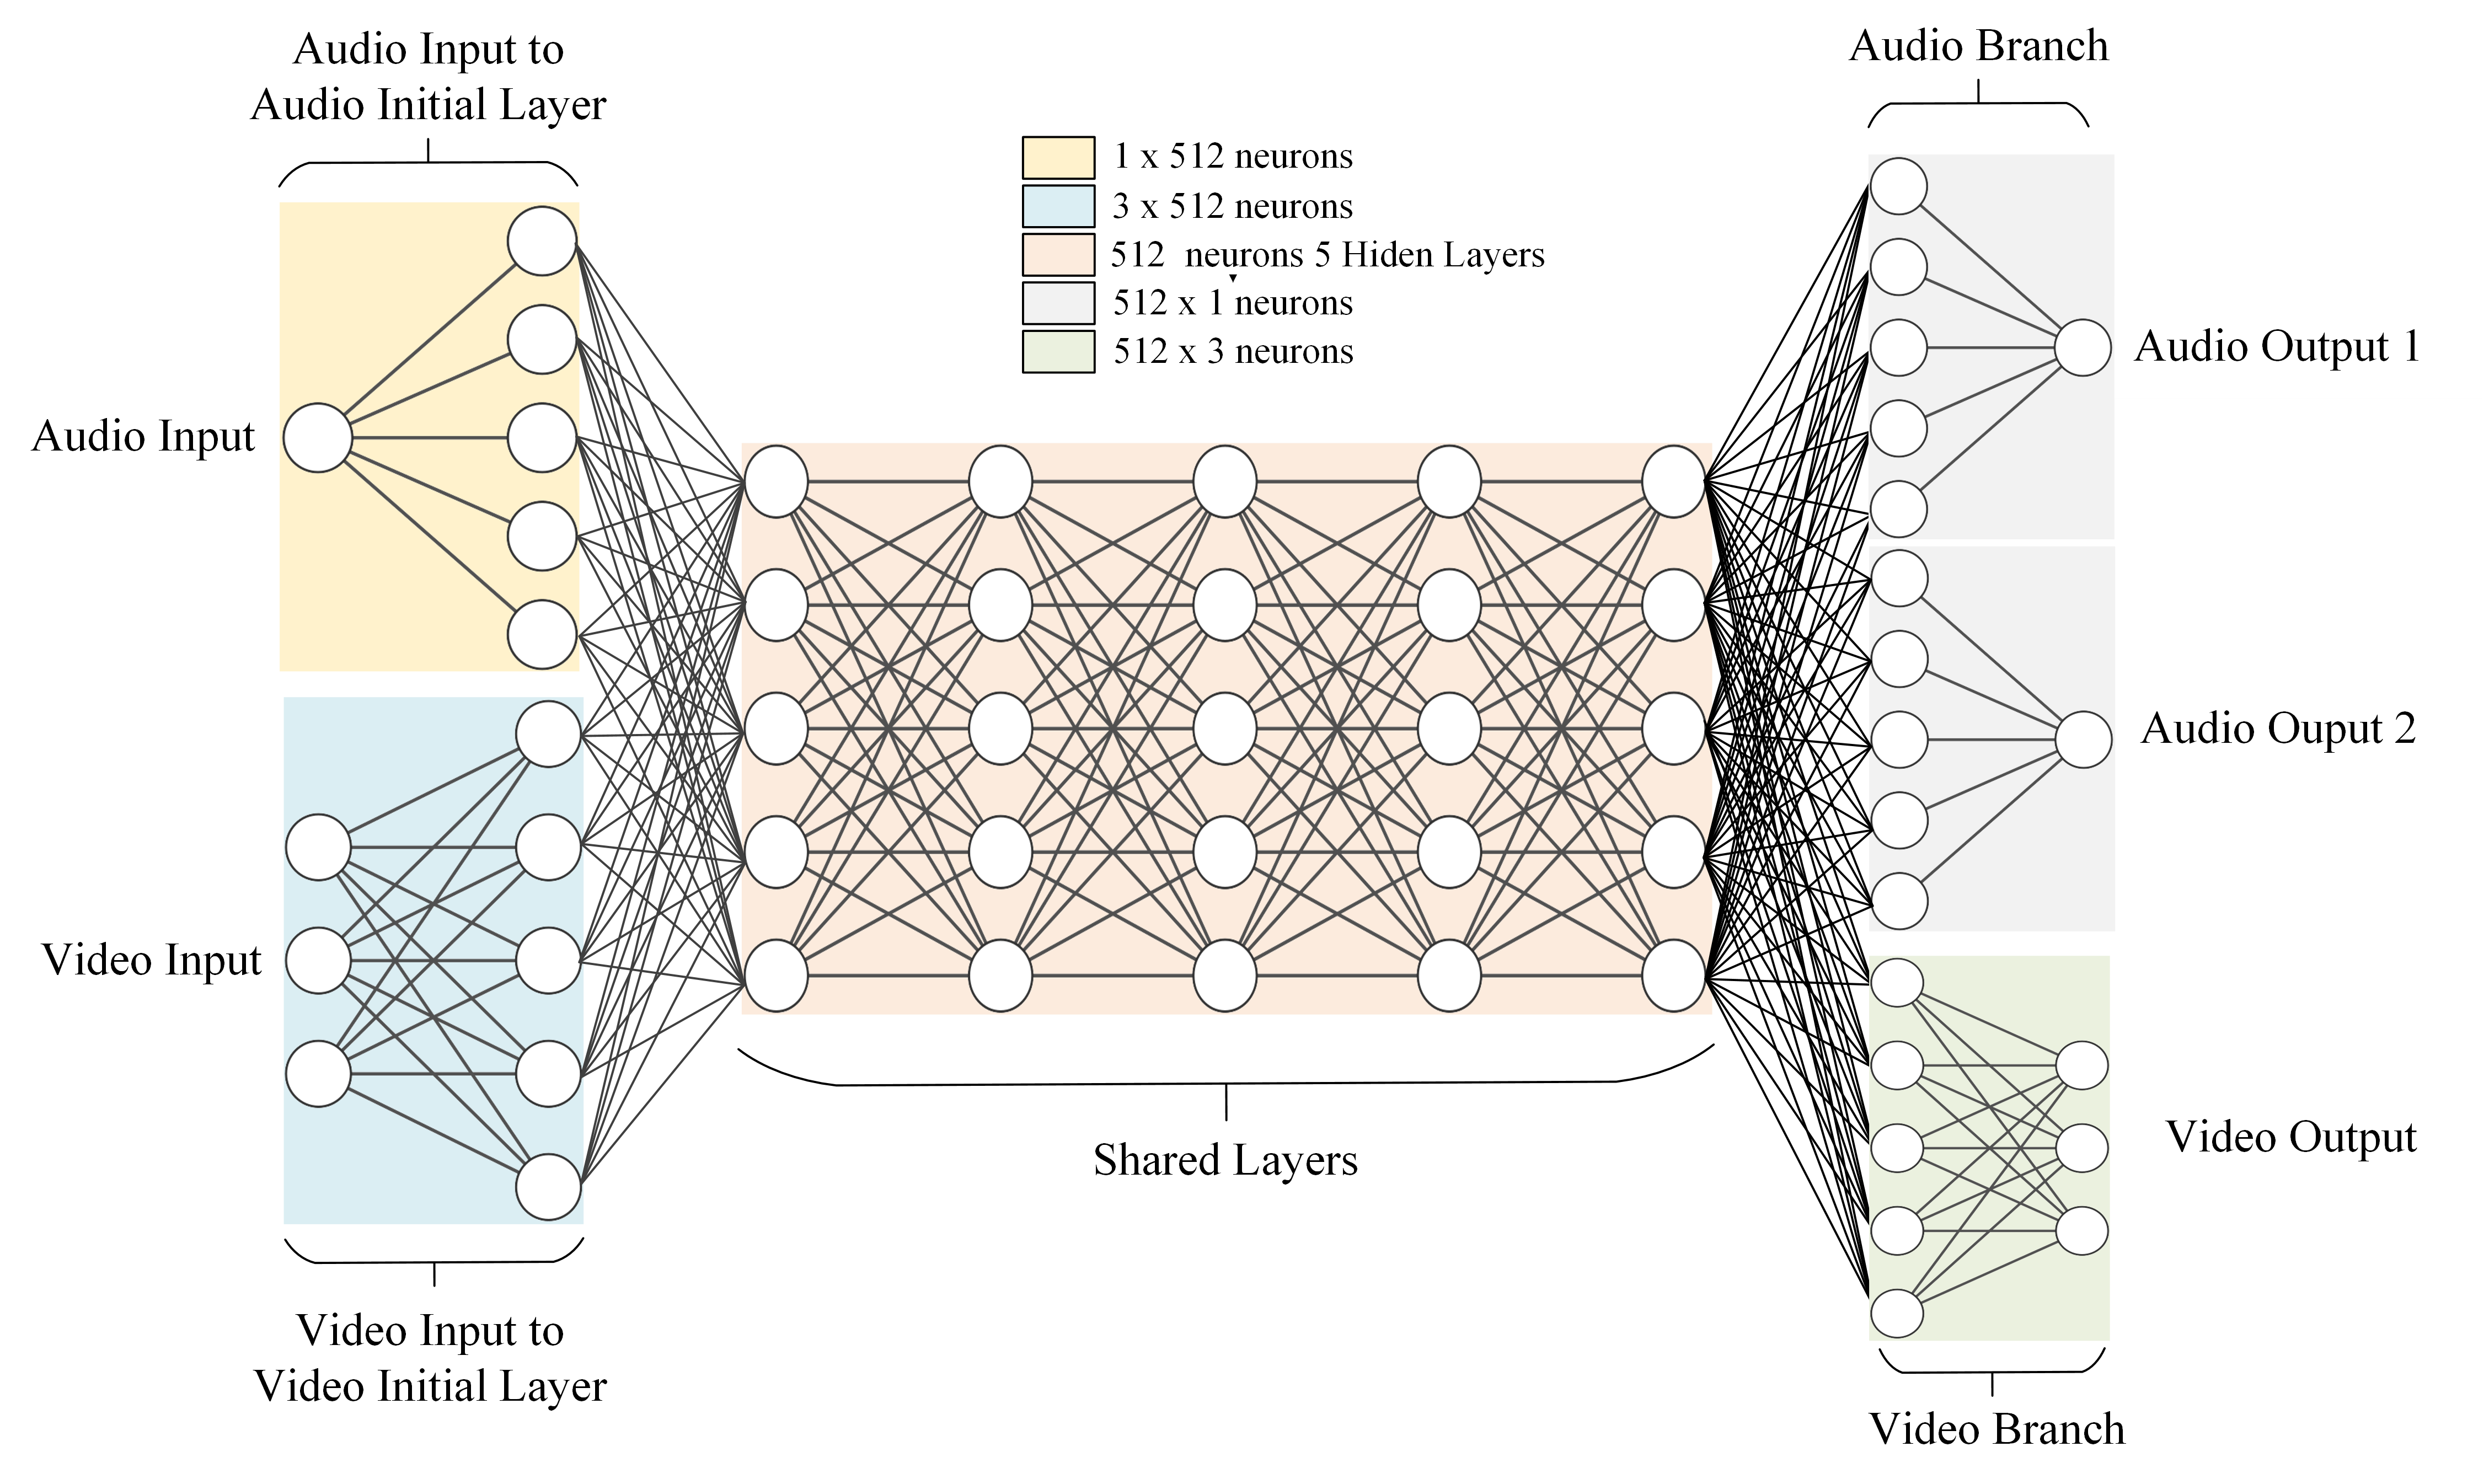
\includegraphics[width=\linewidth]{assets/audio_video_neural.png}
    \caption{SIREN Architecture for Video with Audio}
    \label{fig:arch-audio}
\end{figure}

The \gls{siren} architecture for video with audio consists of three major components: the initial layers, the shared layers, and the video/audio branches. The input to the network includes the spatial-temporal coordinates \(x, y, t\), the frame index \(t\), and the audio timestep \(T\), while the output consists of the RGB pixel values and the audio amplitude \(A\).

The input \(T\) is passed to the audio initial branch and the  spatial-temporal input \(x, y, t\) is fed into the video initial branch. The outputs from these initial layers are then combined and sent to the shared layers, which consist of five layers for the teacher model and three layers for student.

The output from the shared layers is branched into three separate layers: two branches for audio and one for video. The two audio branches are identical, each comprising one layer, which  is a linear layer. These two branches each produce slightly different amplitudes \(A\) for the same audio timestep \(T\), and these outputs are used to estimate and remove noise from the audio data. The video branch consists of one layer as well, being a linear layer, whose output is the RGB values.

The distinct initial layers for audio and video are necessary because it is not possible to have a good initialization for both audio and video if they were in the same branch. The audio branch works well with weights initialized within the range \([-25, 25]\), and the video branch performs well with weights initialized in the range \([-2/3, 2/3]\). Therefore, separate initial layers are required to optimize the reconstruction quality for both modalities.

The two identical audio branches are crucial because they provide the necessary outputs for noise estimation and removal from the audio data. All hidden layers in the shared and initial branches consist of 512 neurons for teacher model while all layers except hidden layers consists of 300 neurons with hidden layers consisting of 512 neurons for student model, with sine activations, except for the last layers in the two audio output branches and the video output branch, which uses linear activation.

\subsubsection{Trainable Parameters}
The breakdown of the trainable parameters (weights and biases) are as follows:

\begin{table}[H]
    \caption{Trainable Parameters in the SIREN Models}
    \label{table:trainable-parameters-teacher-student}
    \centering
    \resizebox{\textwidth}{!}{
    \begin{tabular}{|p{6em}|l|c|c|c|c|}
    \hline
    \multirow{2}{*}{\textbf{Layer}}             & \multirow{2}{*}{\textbf{Parameter}}             & \multicolumn{2}{c|}{\textbf{Dimensions}} & \multicolumn{2}{c|}{\textbf{Total}} \\ \cline{3-6}
                                  &                                  & \textbf{Teacher}    & \textbf{Student}    & \textbf{Teacher}    & \textbf{Student}    \\ \hline
    \multirow{2}{8em}{\textbf{Audio Initial Branch}} & Weight matrix                   & $1 \times 512$      & $1 \times 300$      & 512                 & 300                 \\
                                  & Bias vector                     & $512$               & $300$               & 512                 & 300                 \\ \hline
    \multirow{2}{8em}{\textbf{Video Initial Branch}} & Weight matrix                   & $3 \times 512$      & $3 \times 300$      & 1,536               & 900                 \\
                                  & Bias vector                     & $512$               & $300$               & 512                 & 300                 \\ \hline
    \multirow{2}{5em}{\textbf{Shared Layers}}        & Weight matrix                   & $1024 \times 512$   & $600 \times 512$    & 524,288             & 307,200             \\
                                  & Bias vector                     & $512$               & $512$               & 512                 & 512                 \\
                                  & Weight matrix        & $4 \times (512 \times 512)$    & $2 \times (512 \times 512)$ & 1,048,576     & 524,288            \\
                                  & Bias vector         & $4 \times 512$      & $2 \times 512$      & 2,048               & 1,024              \\ \hline
    \multirow{2}{5em}{\textbf{Video Branch}}         & Weight matrix                   & $512 \times 512$    & $512 \times 300$    & 262,144             & 153,600             \\
                                  & Bias vector                     & $512$               & $300$               & 512                 & 300                 \\
                                  & Weight matrix                   & $512 \times 3$      & $300 \times 3$      & 1,536               & 900                 \\
                                  & Bias vector                     & $3$                 & $3$                 & 3                   & 3                   \\ \hline
    \multirow{2}{5em}{\textbf{Audio Branch 1}}       & Weight matrix                   & $512 \times 512$    & $512 \times 300$    & 262,144             & 153,600             \\
                                  & Bias vector                     & $512$               & $300$               & 512                 & 300                 \\
                                  & Weight matrix                   & $512 \times 1$      & $300 \times 1$      & 512                 & 300                 \\
                                  & Bias vector                     & $1$                 & $1$                 & 1                   & 1                   \\ \hline
    \multirow{2}{5em}{\textbf{Audio Branch 2}}       & Weight matrix                   & $512 \times 512$    & $512 \times 300$    & 262,144             & 153,600             \\
                                  & Bias vector                     & $512$               & $300$               & 512                 & 300                 \\
                                  & Weight matrix                   & $512 \times 1$      & $300 \times 1$      & 512                 & 300                 \\
                                  & Bias vector                     & $1$                 & $1$                 & 1                   & 1                   \\ \hline
    \multicolumn{4}{|c|}{\textbf{Total}}  & \textbf{2,369,029}  & \textbf{1,298,029} \\ \hline
    \end{tabular}
    }
\end{table}


The total number of trainable parameters in the neural network is 2,369,029 for teacher model and 1,298,029 for student model.

\subsubsection{Hyperparameters for the Model}
\begin{table}[H]
    \centering
    \caption{Hyperparameters for Training the Teacher and Student Models}
    \begin{tabular}{|l|p{0.2\textwidth}|p{0.3\textwidth}|}
    \hline
    \textbf{Hyperparameter ($\boldsymbol{\theta}$)} & \textbf{Teacher Model} & \textbf{Student Model}  \\
    \hline
    Number of Epochs                   & 7000                    & 6000                    \\
    \hline
    \multicolumn{1}{|l|}{Omega ($\omega$)} & \multicolumn{2}{c|}{30}  \\
    \hline
    \multicolumn{1}{|l|}{First Layer Weight (Audio) ($\beta_a$)} & \multicolumn{2}{c|}{$(-25, 25)$} \\
    \hline
    \multicolumn{1}{|l|}{First Layer Weight (Video) ($\beta_v$)} & \multicolumn{2}{c|}{$\left(-\frac{2}{3}, \frac{2}{3}\right)$} \\
    \hline
    Learning Rate ($\eta$)              & $1\times10^{-5}$       & $1\times10^{-4}$ for the first 1000 epochs, $1\times10^{-5}$ for the remaining 5000 epochs \\
    \hline
    \multicolumn{1}{|l|}{Optimizer ($\text{Opt}$)} & \multicolumn{2}{c|}{Adam} \\
    \hline
    \end{tabular}
    \label{tab:teacher_student_model_hyperparams}
\end{table}
    
The model was trained for 7000 epochs for the teacher model and 6000 epochs for the student model, with the best-performing version saved based on the lowest loss achieved during training. The value of $\omega$ was set to 30 for both models, following the default configuration of the \gls{siren}model, as it effectively balances frequency representation.

For the first layer weight initialization, the audio branch used a range of $(-25, 25)$ ($\beta_a$) for both the teacher and student models. This range was specifically chosen to accurately represent high-frequency audio features while avoiding unnecessary noise. Larger ranges were tested but resulted in excessive noise, making $(-25, 25)$ the ideal choice.

Similarly, the video branch utilized a narrower initialization range of $\left(-\frac{2}{3}, \frac{2}{3}\right)$ ($\beta_v$) for both models, reflecting the lower frequency nature of video data. Wider ranges led to grainy images and inaccurate color predictions, confirming this range as optimal.

The learning rate was set to $1 \times 10^{-5}$ ($\eta$) for the teacher model and $1 \times 10^{-4}$ for the first 1000 epochs, then $1 \times 10^{-5}$ for the remaining 5000 epochs for the student model, ensuring stable and gradual optimization without large fluctuations in the loss function. The Adam optimizer ($\text{Opt}$) was employed for both models, due to its suitability for SIREN-based models, leveraging its adaptive learning capabilities to efficiently handle sinusoidal feature extraction and optimize the model effectively.

\pagebreak

\subsection{Data Preparation and Training Implementation}

\subsubsection{Pseudocode for Data Preparation}

\autoref{alg:synchronize_video_audio} ensures that the total number of video pixels and corresponding audio samples are synchronized for input compatibility with the model, which requires inputs in the format \([(x, y, t), T]\). 

If the number of video samples (\texttt{video\_size}) is less than the number of audio samples (\texttt{audio\_size}), the algorithm repeats the video coordinates and data until they match the audio sample count. The repetition is performed by calculating a repeat factor as the integer division of \texttt{audio\_size} by \texttt{video\_size}, and appending any remaining samples as needed. 

Similarly, if the audio sample count is smaller, the audio coordinates and data are repeated to align with the video sample count. The process ensures that both video and audio inputs are synchronized and ready for processing by the model.

The synchronized outputs are returned as \texttt{video\_coords}, \texttt{video\_data}, \texttt{audio\_coords}, and \texttt{audio\_data}.

\begin{algorithm}
    \caption{Synchronize Video and Audio Samples}
    \label{alg:synchronize_video_audio}
    \begin{algorithmic}[1]
    \REQUIRE video\_coords, video\_data, audio\_coords, audio\_data
    \STATE video\_size $\gets$ Number of video samples
    \STATE audio\_size $\gets$ Number of audio samples
    \IF{video\_size \textless\ audio\_size}
        \STATE repeat\_factor $\gets \lfloor$ audio\_size / video\_size $\rfloor$
        \STATE remainder $\gets$ audio\_size mod video\_size
        \STATE Repeat video coordinates and data by repeat\_factor
        \IF{remainder \textgreater\ 0}
            \STATE Append first remainder video samples
        \ENDIF
    \ELSIF{audio\_size \textless\ video\_size}
        \STATE repeat\_factor $\gets \lfloor$ video\_size / audio\_size $\rfloor$
        \STATE remainder $\gets$ video\_size mod audio\_size
        \STATE Repeat audio coordinates and data by repeat\_factor
        \IF{remainder \textgreater\ 0}
            \STATE Append first remainder audio samples
        \ENDIF
    \ENDIF
    \RETURN Synchronized video\_coords, video\_data, audio\_coords, audio\_data
    \end{algorithmic}
\end{algorithm}

\autoref{alg:load_video_audio} prepares ground truth data and input coordinates for the model. It loads and normalizes video and audio data from the provided paths, generating spatial (x, y) and temporal (frame index, time) coordinates. Video and audio are synchronized using \autoref{alg:synchronize_video_audio}, ensuring alignment between frames and audio samples. The combined coordinates and normalized data are returned as the final input for the model.

\begin{algorithm}
    \caption{Load and Prepare Video with Audio Data}
    \label{alg:load_video_audio}
    \begin{algorithmic}[1]
    \REQUIRE path\_to\_video, path\_to\_audio, sidelength
    \STATE \textbf{Load Video Data:}
    \IF{path\_to\_video contains '.npy'}
        \STATE video\_data $\gets$ Load data using NumPy
    \ELSIF{path\_to\_video contains '.mp4' \OR path\_to\_video contains '.avi'}
        \STATE video\_data $\gets$ Read frames using skvideo.io.vread
        \STATE Normalize video\_data $\gets$ video\_data / 255.0
    \ENDIF
    \STATE video\_shape $\gets$ (frames, height, width)
    \STATE channels $\gets$ RGB channels of video\_data
    
    \STATE \textbf{Load or Extract Audio Data:}
    \IF{path\_to\_audio contains '.mp4' \OR path\_to\_audio contains '.avi'}
        \STATE Extract audio using FFmpeg and save as a temporary .wav file
        \STATE audio\_rate, audio\_data $\gets$ Load .wav file using wavfile.read
        \STATE Remove the temporary .wav file
    \ELSE
        \STATE audio\_rate, audio\_data $\gets$ Load directly using wavfile.read
    \ENDIF
    \STATE Normalize audio\_data $\gets$ audio\_data / max(abs(audio\_data))
    
    \STATE Compute audio\_samples\_per\_frame $\gets$ len(audio\_data) / Number of video frames
    
    \STATE \textbf{Generate Video Coordinates:}
    \STATE mgrid\_video $\gets$ Generate (x, y) grid for each frame using get\_mgrid
    \STATE Normalize frame indices frameindex $\gets$ linspace(0, 1, Number of frames)
    \STATE Repeat (x, y) coordinates for all frames and append frameindex
    \STATE video\_coords $\gets$ Flattened (x, y, frameindex)
    \STATE Flatten video\_data $\gets$ Normalize and reshape to (N, channels)
    
    \STATE \textbf{Generate Audio Coordinates:}
    \STATE Normalize time audio\_coords $\gets$ linspace(0, 1, len(audio\_data))
    \STATE Flatten audio\_data $\gets$ Reshape to (N, 1)
    
    \STATE \textbf{Synchronize Video and Audio:}
    \STATE (video\_coords, video\_data, audio\_coords, audio\_data) $\gets$ \textbf{\autoref{alg:synchronize_video_audio}}
    
    \STATE \textbf{Combine Video and Audio Data:}
    \STATE combined\_coords $\gets$ Concatenate video\_coords and audio\_coords
    \STATE combined\_data $\gets$ Concatenate video\_data and audio\_data
    
    \RETURN (combined\_coords, combined\_data)
    \end{algorithmic}
\end{algorithm}

\pagebreak 

\subsubsection{Pseudocode for Training}
The following algorithms describe training the teacher and student models using knowledge distillation, where the teacher guides the student to achieve efficient performance by transferring knowledge.

\begin{algorithm}
    \caption{Training the Teacher Model}
    \label{alg:teacher-train-loop}
    \begin{algorithmic}[1]
        \REQUIRE Dataset \texttt{D}, model \texttt{M}, optimizer \texttt{O}, hyperparameters: epochs \texttt{N}, learning rate \texttt{lr}, batch size \texttt{B}, best loss \texttt{best\_loss}
    
        \STATE Initialize dataset \texttt{D}, DataLoader \texttt{D\_loader}, and model \texttt{M}.
        \STATE Initialize optimizer \texttt{O} with learning rate \texttt{lr}.
        \STATE Set the number of epochs \texttt{epochs = N} and initialize \texttt{best\_loss = +$\infty$}.
    
        \FOR{epoch \texttt{i} = 1 \texttt{to} \texttt{N}}
            \STATE Sample a batch \texttt{(inputs, targets)} from \texttt{D\_loader}.
            \STATE Move data to device: \texttt{inputs, targets}.
    
            \STATE \textbf{Step 1: Model Inference}
            \STATE Compute model outputs:
            \[
            \hat{y} = M(x)
            \]
    
            \STATE \textbf{Step 2: Compute Loss}
            \STATE Compute the loss function:
            \[
            L = \lambda_1 \cdot \text{MSE}(\hat{y}_\text{video}, y_\text{video}) + \lambda_2 \cdot \text{MSE}(\hat{y}_\text{audio}, y_\text{audio})
            \]
         
    
            \STATE \textbf{Step 3: Backpropagation and Optimization}
            \STATE Zero gradients and perform backpropagation:
            \[
            \nabla_{\theta} L
            \]

            \STATE Update model parameters:
            \[
            \theta \gets \theta - \eta \cdot \nabla_{\theta} L
            \]
    
            \STATE \textbf{Step 4: Save Best Model}
            \IF{\texttt{L < best\_loss}}
                \STATE Save the model weights and update best\_loss.
            \ENDIF
    
            \STATE \textbf{Step 5: Log Training Progress}
            \STATE Log or print current loss and training progress.
        \ENDFOR
    \end{algorithmic}
\end{algorithm}

\autoref{alg:teacher-train-loop} describes the training process for the teacher model. It initializes the dataset, model, optimizer, and training parameters such as learning rate. During training, batches of input data and their corresponding targets are sampled and used for inference. The model computes outputs, calculates the loss based on \gls{mse} for both video and audio components, and updates its weights using backpropagation. 

\autoref{alg:student-train-loop} outlines training the student model using knowledge distillation. It leverages a pretrained teacher model to guide the learning of the student model.
\begin{algorithm}[ht!]
    \caption{Training the Student Model Using a Teacher Model}
    \label{alg:student-train-loop}
    \begin{algorithmic}[1]
        \REQUIRE Pretrained teacher model \texttt{T}, student model \texttt{S}, dataset \texttt{D}, optimizer, hyperparameters: epochs \texttt{N}, learning rate \texttt{$\eta$}, weight \texttt{$\alpha$}
    
        \STATE Load the dataset \texttt{D} and prepare a data loader.
        \STATE Load teacher model \texttt{T} with pretrained weights.
        \STATE Initialize student model \texttt{S} and optimizer with learning rate \texttt{$\eta$}.
    
        \FOR{each epoch \texttt{$i = 1, \dots, N$}}
            \STATE Sample a batch \texttt{(x, y)} from the data loader, where \texttt{x} is the input and \texttt{y} is the ground truth.
            \STATE Move data \texttt{(x, y)} to the computation device (e.g., GPU).
    
            \STATE \textbf{Step 1: Teacher Model Inference}
            \STATE Compute teacher outputs:
            \[
            \hat{y}_T = T(x)
            \]
    
            \STATE \textbf{Step 2: Student Model Inference}
            \STATE Compute student outputs:
            \[
            \hat{y}_S = S(x)
            \]
    
            \STATE \textbf{Step 3: Compute Losses}
            \STATE Split ground truth \texttt{y} into components (e.g., \texttt{y = (y\_video, y\_audio)}).
            \STATE Compute the hard loss (comparison with ground truth):
            \[
            L_\text{hard} = \beta_1 \cdot \text{MSE}(\hat{y}_S^\text{video}, y_\text{video}) + 
                            \beta_2 \cdot \text{MSE}(\hat{y}_S^\text{audio}, y_\text{audio})
            \]

            \STATE Compute the soft loss (comparison with teacher outputs):
            \[
            L_\text{soft} = \gamma_1 \cdot \text{MSE}(\hat{y}_S^\text{video}, \hat{y}_T^\text{video}) +
                            \gamma_2 \cdot \text{MSE}(\hat{y}_S^\text{audio}, \hat{y}_T^\text{audio})
            \]

            \STATE Combine hard and soft losses:
            \[
            L_\text{total} = \alpha \cdot L_\text{hard} + (1 - \alpha) \cdot L_\text{soft}
            \]
    
            \STATE \textbf{Step 4: Update Student Model}
            \STATE Perform backpropagation and update \texttt{S}:
            \[
            \theta_S \gets \theta_S - \eta \cdot \nabla_{\theta_S} L_\text{total}
            \]
    
            \STATE \textbf{Step 5: Save Best Model (if applicable)}
            \IF{$L_\text{total} < L_\text{best}$}
                \STATE Save \texttt{S} and update \texttt{$L_\text{best}$}.
            \ENDIF
    
            \STATE Log training progress (e.g., loss values) to a file.
        \ENDFOR
    \end{algorithmic}
\end{algorithm}
The teacher's outputs serve as ``soft targets", in addition to the ``hard targets" from the ground truth. Losses are computed for both soft and hard targets, and a weighted loss drives the student model's optimization enables the student model to mimic the teacher while retaining its own efficiency.

\subsection{LZMA2 Compression of Model}
\begin{algorithm}
    \caption{LZMA2 Compression Algorithm}
    \label{alg:lzma2-compression}
    \begin{algorithmic}[1]
    \REQUIRE input\_data, dictionary\_size, compression\_level
    \STATE Initialize dictionary with size dictionary\_size
    \STATE Configure compression parameters based on compression\_level
    \STATE Initialize range encoder and output buffer
    \STATE pos $\gets$ 0
    \WHILE{pos $<$ len(input\_data)}
        \STATE Determine block\_size based on remaining data and performance criteria
        \STATE Evaluate compression gain for the current block
        \IF{compression gain is insufficient}
            \STATE \textbf{Set Block Type:} Uncompressed
            \STATE Write control byte with uncompressed flag and block\_size to output buffer
            \STATE Copy raw data block from input\_data[pos : pos+block\_size] to output buffer
        \ELSE
            \STATE \textbf{Set Block Type:} Compressed
            \STATE Write control byte with compressed flag and block\_size to output buffer
            \FOR{each position \texttt{i} in input\_data[pos : pos+block\_size]}
                \STATE Search dictionary for the longest match for input\_data[i:]
                \IF{match is found}
                    \STATE Encode match length and distance using range encoder
                    \STATE Update dictionary with matched sequence
                    \STATE Advance \texttt{i} by match length
                \ELSE
                    \STATE Encode literal byte input\_data[i] using range encoder
                    \STATE Update dictionary with literal byte
                    \STATE Advance \texttt{i} by 1
                \ENDIF
            \ENDFOR
            \STATE Append encoded block from range encoder to output buffer
        \ENDIF
        \STATE Update pos $\gets$ pos + block\_size
    \ENDWHILE
    \STATE Write end-of-stream marker to output buffer
    \RETURN compressed\_data from output buffer
    \end{algorithmic}
\end{algorithm}

\autoref{alg:lzma2-compression} outlines the abstract LZMA2 compression process. The algorithm begins by initializing a dictionary and configuring the compression parameters based on the desired compression level. It then iterates over the input data in blocks, dynamically deciding whether to compress a block or store it uncompressed based on the potential compression gain. For compressed blocks, the algorithm performs match searching within the dictionary, encoding matches and literal bytes via a range encoder. Finally, it writes an end-of-stream marker and returns the assembled compressed data.

\pagebreak 
